\section{Model architecture and training}

\subsection{Model architecture}



\if false
===OLD SRP CONTENT===
This chapter describes the architecture of the neural models used to calculate a similarity score, i.e. the semantic relatedness, for a given sentence tuple and how these models are trained. 

%\todo{UL: Hier wäre mehr Übersicht gut: was kommt jetzt? Was wurde gemacht? Was davon ist neu? Was ist das Ziel? (X)}  \todo{AB: introduce the two parameters!}
As we intend to analyze the impact of dependency type information and order aware processing, we introduce two boolean parameters, \texttt{dependency available} and \texttt{order aware}, to indicate if the respective information is exploited. After introducing the general model architecture, we explain how these parameters are realized. Then, we describe the baseline model and finally name implementation and training details.


\subsection{Model architecture} \label{subsec:architecture}
Both models consist of a sentence embedding unit and a similarity function. The embedding unit translates a sequence of tokens into a single embedding vector and is applied to the two input sentences using identical weights, thus our systems follow a siamese structure \autocite{bromley_signature_1994}. %\textcite{he_multi-perspective_2015}: "Our model has a “Siamese” structure (Bromley et al., 1993) with two subnetworks each processing a sentence in parallel. The subnetworks share all of their weights, and are joined by the similarity measurement layer, then followed by a fully connected layer for similarity score output."
They calculate the sentence embedding by gathering the individual embeddings for the contained tokens, eventually enhancing them with additional information, and applying a composition function. The two resulting embeddings are fed into the similarity function that produces the similarity score. 

Figure~\ref{fig:model_architecture} shows this architecture. In the following, we describe the respective modules. 

\begin{figure}[htb!]
	\centering
	%\textbf{Deviations from gold score}\par\medskip
	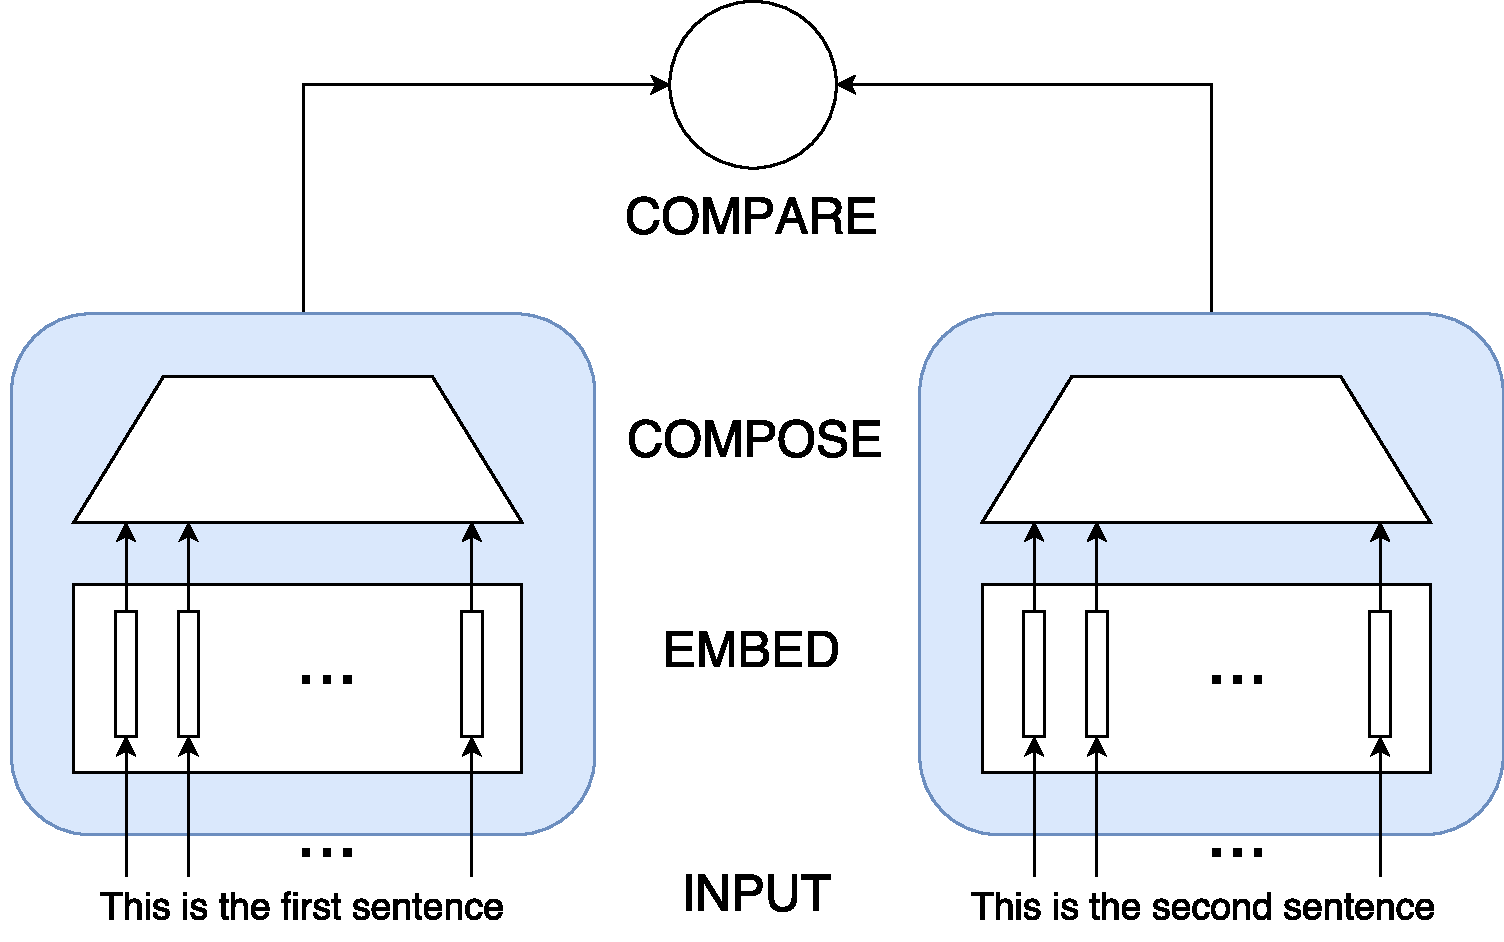
\includegraphics[width=.8\linewidth]{model/SA_model.pdf}
	\caption{General architecture. The functionality marked by the blue boxes is identical for both input sentences, i.e. they share structure and weights.}
	\label{fig:model_architecture}
\end{figure}

\subsubsection{Token Embeddings}
%see naili_comparative_2017
We use 300 dimensional %\todo{UL: precomputed? on which data? (X)} 
GloVe vectors \autocite{pennington_glove_2014} pretrained on the Common Crawl\footnote{see \url{http://commoncrawl.org}} corpus to embed individual word tokens as they show good performance on several \ac{NLP} tasks and perform comparable to its major competitor, Word2Vec \autocite{levy_improving_2015,naili_comparative_2017}. To evaluate the influence of dependency types, we concatenate the embedding with the one-hot encoded dependency type (Section~\ref{subesec:training_implementation}). %\todo{UL: welcher Parser?(X) erwartete Genauigkeit?}. 
The dependency type tag set is based on the Universal Dependencies project \autocite{nivre_universal_2016} and includes 40 different types, resulting in 340 dimensional vectors as input for the composition function. When disabling this feature, we set these 40 entries to zero. The token embeddings are not optimized during training of our models.   

\subsubsection{Composition function}
We compare two composition functions: (1) \acf{AVG} and (2) \acf{LSTM}. 
In the \ac{AVG} case, we apply one \acf{FC} with $tanh$ as activation function to every token embedding. Then, averaging the resulting vectors gives the sentence embedding.
In the \ac{LSTM} setting, the token embeddings are fed directly into a LSTM layer whose final state \todo{UL: remove "final state" (?)} output is used as sentence embedding. %The two settings are visualized in Figure~\todo{AB: add figure}.

To achieve comparability between the two composition functions, we control the amount of effectively trainable parameters in each of them. Depending on whether dependency type information is used, we use different sizes for the $tanh$ \ac{FC} in the \ac{AVG} case and for the inner state of the \ac{LSTM} to fix the amount of effective parameters. Table~\ref{tab:sizes} shows the exact numbers and sizes of the elements. The sentence representation dimension equals to the composition element (output) size.  % total sizes: AVG=input*fc, LSTM=(input+state+1)*4*state 

\begin{table}[!htb]
  \centering
  \begin{tabular}{ l | c | c }
      & AVG (FC size) & LSTM (state size) \\ \hline
    w/ dependency types & 110840 (326) & 111248 (68) \\ 
    w/o dependency types & 111000 (370) & 111000 (74) \\
  \end{tabular}
  \caption{Numbers of trainable parameters and (output) size of composition function elements}
  \label{tab:sizes}
\end{table}

\subsubsection{Similarity calculation}
We use the cosine similarity to calculate the similarity score between the two sentence embeddings as described in section~\ref{subsec:similarity_measure}.
%\begin{equation}
%f_{SIM_{cos}}(a,b) = \frac{a \cdot b}{\norm{a}_2\norm{b}_2} 
%\end{equation}

\subsection{Baseline model}
As baseline we calculate TF-IDF based similarity scores in the following manner. We parse and lemmatize each sentence and filter for verbs, nouns and adjectives according to POS tags. Then, we embed each sentence with TF-IDF as described in section~\ref{subsec:doc_embedding} and apply cosine measure. 

\subsection{Implementation and Training}
\label{subesec:training_implementation}
The model is implemented with the TensorFlow framework  \autocite{abadi_tensorflow_2016}. TensorFlow allows to define and to execute arbitrary dataflow graphs efficiently on different devices as CPUs or GPUs. For tokenization, dependency parsing and POS-tagging we use spaCy\footnote{see \url{https://spacy.io/}} which is a fast and still accurate\footnote{see \textcite{choi_it_2015} for a comparative study} \ac{NLP} framework (labeling score of 93.3\% for dependency parsing, see Section~\ref{subsubsec:dependency_parsing}). 

We train the model via batched back-propagation using \ac{MSE} loss function as described in section~\ref{subsec:cost_function} and apply ADAM \autocite{kingma_adam_2014} %ADADELTA \autocite{zeiler_adadelta_2012}
as optimizer. We use a 4:1:5 train/dev/test split. The training is terminated when the score on the development data set does not increase anymore regarding a smoothing window covering the last 25 epochs.


%\subsection{Pre-Training}
%To increase the amount of available training examples, we examined pre-training on a dataset that is one order of magnitude larger than the SICK corpus. We train the models on this data until the early stopping criterion is met and use the resulting weights to initialize the models trained on the SICK dataset. 

\fi


